
%---------------------- chap 1 ----------------------
\cchapter{مقدمه}
\pagebreak

یکی از مسایل همواره محبوب و چالش‌برانگیز در علم رباتیک، خودروهای هوشمند و هم‌یاری راننده می‌باشد. در اواخر دهه‌ی هشتاد، با ارایه‌ی اولین خودروی بدون سرنشین توسط شرکت \lr{Mercedes-Benz} که از علم بینایی ماشین استفاده می‌کرد
%\cite{benz}
، توجه پژوهشگران زیادی به مسایل گوناگون بینایی ماشین در این زمینه جلب شده‌است. 

یکی از مسایل چالش‌برانگیز در خودروهای هوشمند و نیز هم‌یاری راننده‌، تشخیص تابلوهای راهنمایی و رانندگی می‌باشد. \cite{Gonzalez2014}. در شکل
\ref{fig:signs} 
 تفاوت این دو دسته از تابلوها را مشاهده می‌کنید.


\begin{figure}[t]
\centering
    	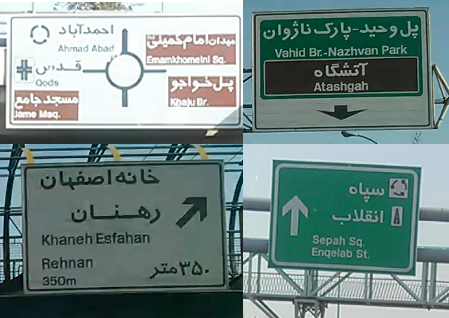
\includegraphics[height=6cm]{Figures/Panels.png}
	   	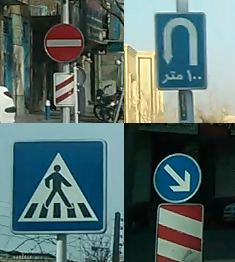
\includegraphics[height=6cm]{Figures/Signs.png}
%برای آن که کپشن تصویر در فهرست شکل‌ها به گونه دیگری بیاید:
\caption[تابلوی راهنما و علایم رانندگی]{راست: تابلوهای راهنما. چپ: علایم راهنمایی و رانندگی. }
\label{fig:signs}
\end{figure}

لورم ایپسوم ( به انگلیسی \lr{lorem ipsum} ) متنی بی مفهوم است که تشکیل شده از کلمات معنی دار یا بی معنی کنار هم. کاربر با دیدن متن لورم ایپسوم تصور میکند متنی که در صفحه مشاهده میکند این متن واقعی و مربوط به توضیحات صفحه مورد نظر است واقعی است. حالا سوال اینجاست که این متن « لورم ایپسوم » به چه دردی میخورد و اساسا برای چه منظور و هدفی ساخته شده است؟ پیش از بوجود آمدن لورم ایپسوم ، طراحان وب سایت در پروژه های وب سایت و طراحان کرافیک در پروژه های طراحی کاتولوگ ، بروشور ، پوستر و ... همواره با این مشکل مواجه بودند که صفحات پروژه خود را پیش از آنکه متن اصلی توسط کارفرما ارائه گردد و در صفحه مورد نظر قرار گیرد چگونه پر کنند؟؟ اکثر طراحان با نوشتن یک جمله مانند «این یک متن نمونه است» ویا «توضیحات در این بخش قرار خواهند گرفت» و کپی آن به تعداد زیاد یک یا چند پاراگراف متن میساختند که تمامی متن ها و کلمات ، جملات و پاراگراف ها تکراری بود و از این رو منظره خوبی برای بیننده نداشت و ضمنا به هیچ وجه واقعی به نظر نمیرسید تا بتواند شکل و شمایل تمام شده پروژه را نشان دهد. از این رو متنی ساخته شد که با دو کلمه ( به فارسی : لورم ایپسوم ) آغاز میشد وبا همین نام در بین طراحان وب و گرافیک شناخته و به سرعت محبوب شد. وب سایت های سازنده لورم ایپسوم میتوانند هر تعداد کلمه و پاراگراف که بخواهید به صوورت تکراری یا غیر تکراری برایتان بسازند و تحویلتان بدهند تا از آنها در پروژه هایتان استفاده کنید. ( لورم ایپسوم فارسی) متن های لورم ایپسوم را به زبان فارسی و علاوه بر زبان فارسی به انگلیسی ، عربی ، ترکی استانبولی و ... برایتان میسازد. زبان های دیگر نیز رفته رفته به بانک اطلاعاتی لورم ایسپوم فارسی اضافه خواهند شد.  

%--------------------- end of chap 1 ----------------